%Review of timbral control research.
%	Timbre Definition
%	Timbre Spaces (MDS and shit)
%	Audio Features
%	Perceptual Control of Synthesis

\chapter{Timbre}
\label{chap:Timbre}
	There are three properties which describe how a sound is perceived, these being loudness, pitch and timbre. Loudness
	describes the perceived intensity of a sound and pitch its perceived frequency. Timbre then describes any other
	properties of a sound, besides loudness and pitch, which allow it to be distinguished from other sounds
	\citep{mathews1999introduction}. Loudness and pitch are both one dimensional properties allowing sounds to be
	ordered from quiet to loud or low to high pitch. Timbre is a more complex property consisting of multiple dimensions
	\citep{rossing2002the}. There is a large body of research concerning the analysis of timbre, identifying these
	dimensions and their relationships with the acoustic features of a sound.

	Simple descriptions of a sounds timbre involve instrument identification. A sound could be described as `cello-like'
	or `flute-like'. More broadly the class of instrument, string or woodwind, could be used to describe the timbre of a
	sound. While these terms are useful for discussing the instrumentation of pieces they can not be applied generally
	to a wide range of timbres. It is not very useful to describe the timbre of a xylophone as being `not flute-like'.

	More general timbral descriptors directly describe the sound itself rather than the source which produced it. These
	include terms such as bright, rough and sharp. This allows the timbre of different sounds to be compared according
	to these terms \citep{howard2009acoustics}. Sounds can also be ordered in respect to these criteria much like with
	loudness and pitch. For example one could order a set of sounds by how bright they sound.

	Early research into timbre was performed by \citet{helmholtz1875on}. More recent work involves research from various
	fields. Low level features of audio segments can be found using signal analysis techniques. More complicated
	information about the perception of a signal can be discovered through modelling the behaviour of the human hearing
	system. Lastly experiments can be undertaken in which participants listen to audio samples and provide responses
	regarding the timbre of the samples. These responses are then analysed to uncover any correlations between the
	participants responses and lower level features of the audio samples.

	This chapter will review the existing body of timbral research. Section \ref{sec:Timbre-LowLevelFeatures} discusses
	metric which are used to describe the low level features of audio signals. Section
	\ref{sec:Timbre-PsychoacousticPrinciples} covers various models which describe the perception of various auditory
	phenomena. \note{Put in what the rest of the sections are about}.

\section{Low Level Audio Features}
\label{sec:Timbre-LowLevelFeatures}
	A widely cited definition of timbre \citep{ASA1960american} suggests that timbre in influenced by various low level
	features of an audio signal. The spectral content, waveform and temporal characteristics all effect the perceived
	timbre of a sound. Signal analysis techniques can be used to extract information about these elements of a signal.
	A large list of such features feature extraction techniques is given by \citep{peeters2004a}. These features can be
	separated into three categories. Features which describe the properties of a signals waveform and how it evolves
	with time (temporal features), features which describe the frequency content of a signal (spectral features) and
	features which describe how the frequency content of a signal evolves with time (spectro-temporal features). 

	\subsection{Temporal Features}
	\label{sec:Timbre-LowLevelFeatures-Temporal}
		Simple temporal features involve taking statistical measurements, such as mean and variance, of the audio
		samples in a signal. These measures give basic information about the level and variation in a signal but in
		many cases they do not represent a signals properties very well. For example, the mean value of a sinusoidal
		signal over a whole number of cycles is zero. 

		A common technique to extract more meaningful information about a signals level is to use an envelope
		detector. An envelope detector extracts the amplitude envelope of a signal. The amplitude envelope provides
		information about the level of a signal over time. An example amplitude envelope is shown in Figure
		\ref{fig:AmplitudeEnvelope}.

		\begin{figure}[h!]
			\centering
			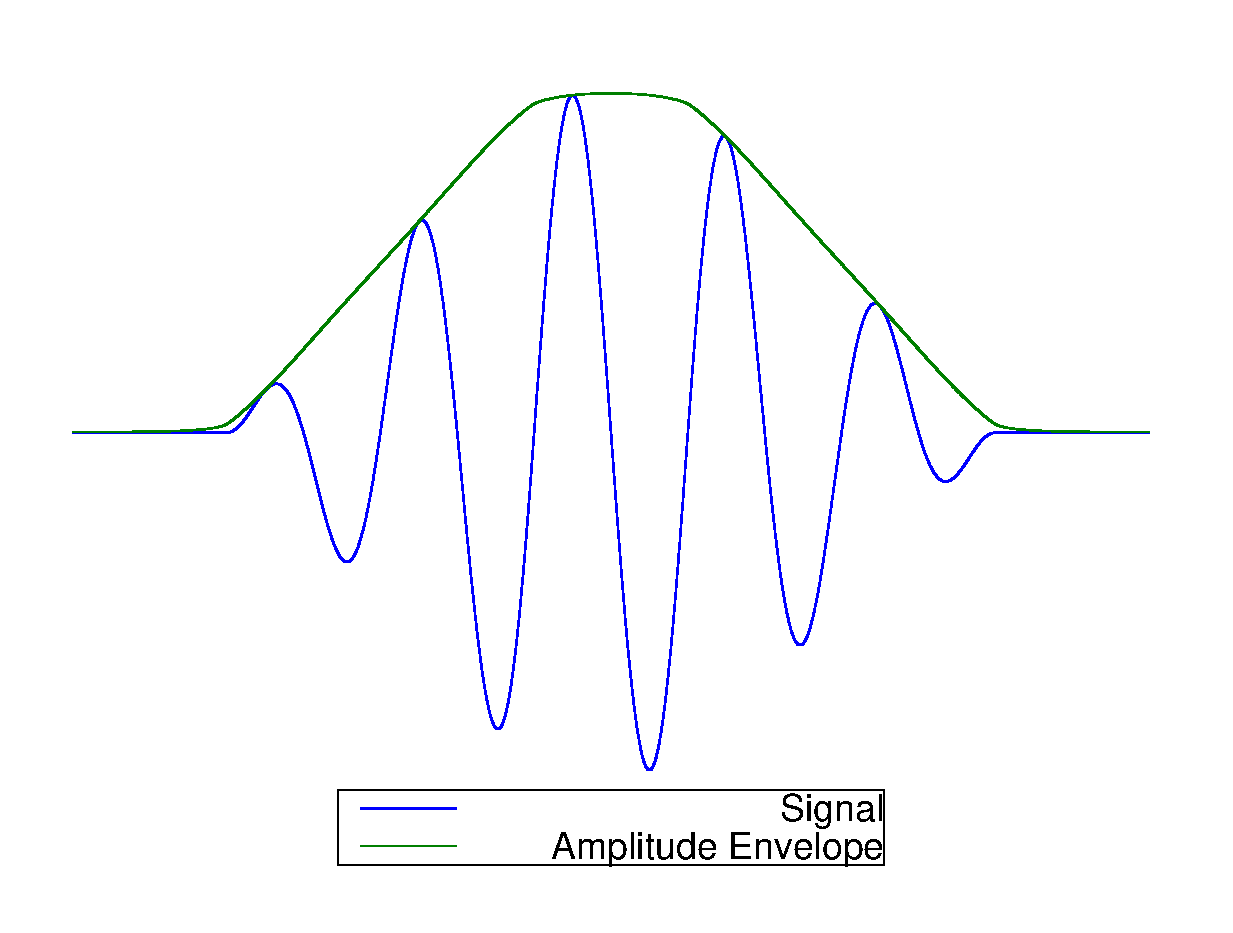
\includegraphics[width=0.6\textwidth]{chapter2/Images/AmplitudeEnvelope.eps}
			\caption{The Amplitude Envelope of a Signal.}
			\label{fig:AmplitudeEnvelope}
		\end{figure}

		Various envelope detection methods are reviewed by \citet{chang2007a}. \citet{howard2009acoustics} separates
		the envelope of a sound into three sections. The steady state section is the middle portion in which the
		timbre of the sound only varies slightly. The onset and offset sections describe the way the sound rises
		from silence to the steady state and returns to silence after. Further refinement of the description of
		amplitude envelopes leads to the ADSR (Attack, Decay, Sustain, Release) model \citep{descrivan2012music}. An
		example ADSR envelope is shown in Figure \ref{fig:ADSR}.

		\begin{figure}[h!]
			\centering
			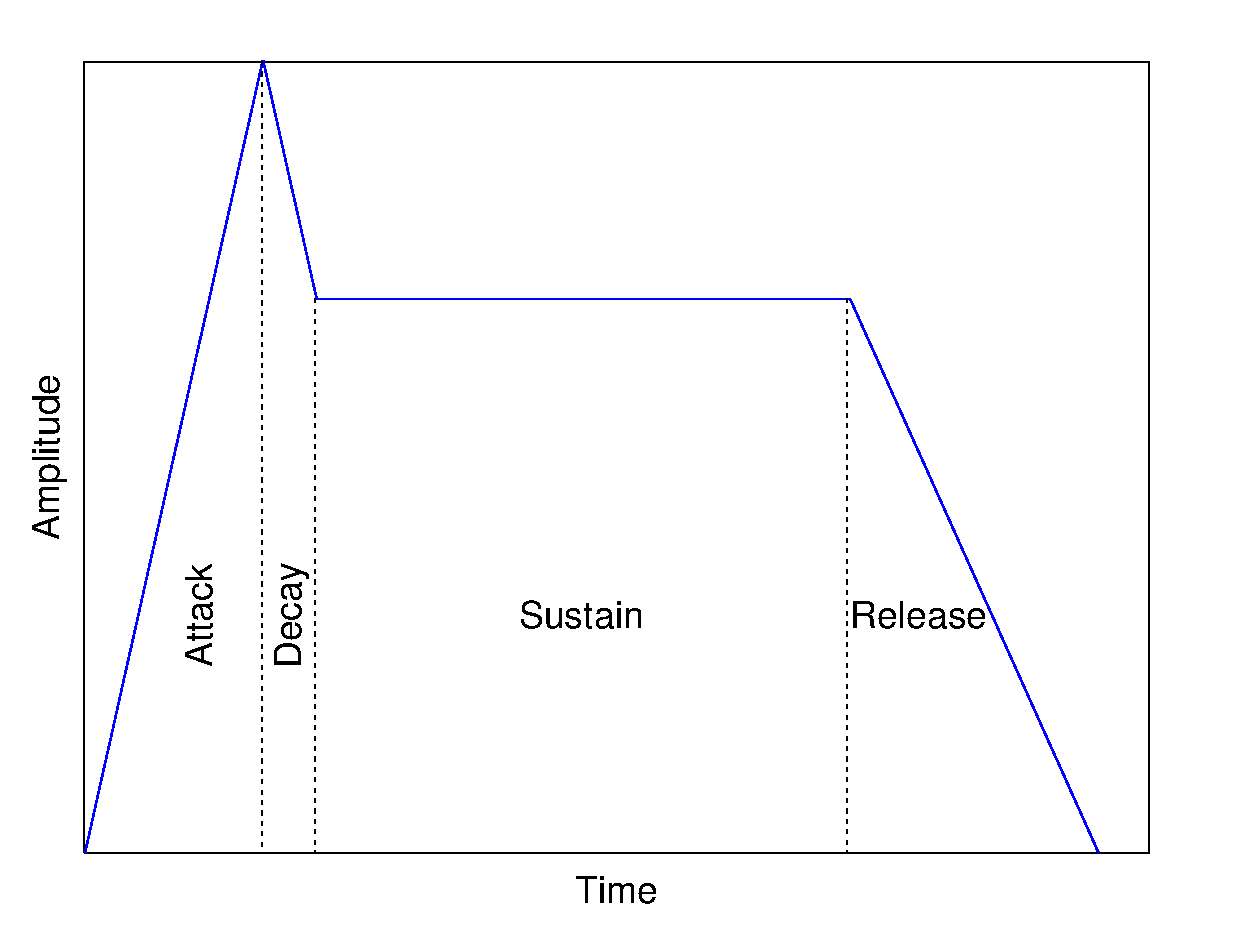
\includegraphics[width=0.6\textwidth]{chapter2/Images/ADSR.eps}
			\caption{An ADSR Envelope.}
			\label{fig:ADSR}
		\end{figure}

		Once the amplitude envelope of a signal has been extracted further statistics can be calculated from it such
		as log attack time and temporal centroid \citep{peeters2000instrument}.

		Some other temporal features measure the oscillation or repetition of a signal. Examples are the zeros
		crossing rate and the autocorrelation, both of which can be used in pitch / frequency estimation
		\citep{mcleod2005a}.

	\subsection{Spectral Features}
	\label{sec:Timbre-LowLevelFeatures-Spectral}
		In existing timbral research is is widely reported that features of a sounds spectrum produce the largest
		effects on timbre. Simple spectral features can be calculated as statistical measures which describe the
		shape of the spectrum. For example the spectral centroid of a signal is calculated as the mean frequency
		weighted by their magnitudes. Spectral centroid is often stated as being one of the most salient audio
		features in timbre recognition \citep{freed1990auditory, lakatos2000a}. Higher order statistical moments of
		the spectrum (standard deviation, skewness and kurtosis) can be used to further describe the distribution of
		energy in the spectrum around the centroid.

		More detailed metrics in the shape of a spectrum can be calculated in the form of Mel Frequency Cepstral
		Coefficients (MFCCs). These measurements were originally used in speech recognition systems
		\citep{davis1980comparison}. More recently they have been applied to the analysis of timbre
		\citep{depoli1997sonological}. 

		Other spectral metrics consider the harmonic structure of a signal. In order to calculate these features the
		partials (prominent frequency components) of the signal must me found. The deviation of these partials from
		perfect harmonic frequencies measures the inharmonicity of the signal. \citet{fletcher1962quality} state
		that inharmonicity of some partials is necessary for the recognition of the timbre of a piano. The noise
		energy in a signal describes any energy which is does not contribute to a partial. The noisiness is then
		measured as the ratio of the noise energy to the total energy in the signal \citep{serra1998sound}.

		Further analysis can be performed by finding the harmonic partials of the signal. In detecting the harmonic
		partials it is usual to allow for a slight deviation from perfect harmonic structure, as described by
		\citet{peeters2011the}. Several metrics have been suggested which constitute the ratio of energy between two
		different sets of harmonic partials. The tristimulus metrics proposed by \citet{pollard1982a} split the
		harmonic series in to three sections, the fundamental frequency, the second through fourth harmonics and,
		the rest of the higher order harmonics. Ratios between each of these sections and the total energy in the
		harmonics are calculated. Another commonly used metric is the ratio between energy in the odd and even order
		harmonic partials. This was found to be a salient feature in the judgement of timbre dissimilarity by
		\citet{hall2010importance}. 

		\note
		{
			Spectro-temporal features exist such as spectral flux.
		}


\section{Psychoacoustic Principles}
\label{sec:Timbre-PsychoacousticPrinciples}
	Psychoacoustics is a field which deals with the perception of sound. The existing literature concerns the study of
	the human hearing system and how it responds to certain aspects of audio stimuli. Several different areas of audio
	perception have been researched. Methods have been devised to model the human perception of loudness
	\citep{moore1997a} and pitch \citep{gerhard2003pitch}. Other research considers the human hearing systems ability to
	locate sound sources \citep{blauert1997spatial}. 

	As discussed in Section \ref{sec:Timbre-LowLevelFeatures-Spectral} there are several metrics to describe the
	spectral content of a signal. While it may be possible to measure changes in values of these features, the changes
	may not be detectable by the human hearing system. Psychoacoustic models allow us to determine how audio signals are
	interpreted by the human hearing system and how well we will notice such changes.

	\subsection{Critical Bands}
	\label{sec:Timbre-PsychoacousticPrinciples-CriticalBands}
		The part of the inner ear which deals with frequency separation is know as the basilar membrane. This is a
		structure which resonates at different frequencies along its length. Low frequencies at one end to high at
		the other. A sinusoidal tone excites a portion of the basilar membrane corresponding to a narrow band of
		frequencies. Two tones whose excitation bands overlap will interfere with how each other are perceived by
		the listener.

		The basilar membrane can be modelled as a filter bank comprised of band pass filters. Each of these
		auditory filters represents the region of the membrane excited by a sinusoidal tone at its centre
		frequency. The bandwidth of these filters is known as the critical bandwidth. Portions of signals will
		interfere with the perception of others which are within one critical bandwidth.
		\citet{glasberg1990derivation} simplify the auditory filters by modelling them as rectangular filters. The
		bandwidth of these filters known as the equivalent rectangular bandwidth (ERB) and can be approximated using
		Equation \ref{eq:ERB}.

		\begin{equation}
			ERB(f_{c}) = 24.7(4.37f_{c} + 1)
			\label{eq:ERB}
		\end{equation}

		Where $f_{c}$ is the center frequency of the auditory filter in kHz and $ERB(f_{c})$ is the equivalent
		rectangular bandwidth, in Hz, at that frequency.

		\citet{howard2009acoustics} discusses the perception of two tones, sounded simultaneously, as they get
		further apart in frequency. When within 15Hz of one another the two tones are perceived as a single sound
		with a sinusoidally varying amplitude. The frequency of this variation is equal to the difference in
		frequency of the tones. As the difference in frequencies gets greater then 15Hz this amplitude modulation
		becomes fast enough for it to be perceived as a roughness in texture rather than `beats' in the amplitude.
		In between 15Hz and the critical bandwidth the perceived sound transitions from a single sound to two
		separate sounds but still with a rough texture. Once the difference in frequencies exceeds the critical
		bandwidth the two tones are perceived as separate smooth tones. These effects are summarised in Figure
		\ref{fig:ToneSeparation}.

		\begin{figure}[h!]
			\centering
			\begin{tikzpicture}

				\draw [thick, ->] (0, 0) -- (10, 0);
				\draw (0, 1) -- (10, 1);
				\draw (0, 0) -- (0, 2) -- (10, 2);

				\draw (0, 0) -- (0, -2pt) node [anchor=north] {0};
				\draw (2, 0) -- (2, -2pt) node [anchor=north] {15};
				\draw (8, 0) -- (8, -2pt) node [anchor=north] {CB};

				\fill [pattern=north west lines] (1.75, 0) rectangle (2.25, 1);
				\fill [pattern=north west lines] (7.75, 0) rectangle (8.25, 1);
				\fill [pattern=north west lines] (5.75, 1) rectangle (6.25, 2);

				\node at (0.875, 0.5) {Beats};
				\node at (5, 0.5) {Rough};
				\node at (9.125, 0.5) {Smooth};
				\node at (2.875, 1.5) {Fused};
				\node at (8.125, 1.5) {Separate};

				\node at (5, -1) {Frequency Difference (Hz)};

			\end{tikzpicture}
			\caption{The perceived of two tones as they move further apart in frequency. Hashed areas represent
				 the transition between perceived effects. CB denotes the critical bandwidth.}
			\label{fig:ToneSeparation}
		\end{figure}

		It is evident from Equation \ref{eq:ERB} that the critical bandwidth increases with frequency. This together
		with the perceptual information shown in Figure \ref{fig:ToneSeparation} suggests that tones separated by
		the same amount will be heard as separate if they or both low in frequency but as their frequencies rise
		they will start to be perceived as a single fused sound.

	\subsection{Specific Loudness}
	\label{sec:Timbre-PsychoacousticPrinciples-SpecificLoudness}
		In hearing models for measuring loudness it is common to split the audible spectrum into bands which all
		have the same perceived width. Before calculating the total loudness the specific loudness for each of these
		bands is calculated. The procedure for doing this is beyond the scope of this report. A description of this
		process is provided by \citet{moore1997a}. The specific loudness measures the perceived loudness of a signal
		in a given frequency range. For the analysis of the perception of timbre this allows for better modelling of
		what portions of a signals spectrum are audible. While the spectrum describes what frequency content is
		present in the signal, the specific loudness describes how much of each frequency is perceived by a
		listener.

		A widely used set of bands was proposed by \citet{zwicker1961subdivision} who spilt the spectrum into 24
		bands, each one critical bandwidth wide. These bands are known and the bark bands and provide a perceptual
		unit of frequency, the bark. Integer values of barks occur at the boundaries between two bark bands. An
		change in frequency of one bark is equal to one critical bandwidth.

	\note
	{
		Perhaps some more on masking. Although it may be wasted space.
	}

\section{Timbral Features}
\label{sec:Timbre-TimbralFeatures}
	Models have been developed in the literature to describe certain aspects of the timbre of a sound. Two such models
	are those for describing auditory sharpness and roughness.
	
	\subsection{Sharpness}
		\citet{fastl2007psychoacoustics} discuss the factors leading to the perception of sharpness. The sharpness
		of a signal depends on the ratio of high and low frequency content. Increasing the amount of high frequency
		content increases the sharpness of a signal. The sharpness can also be reduced by adding more low frequency
		content to a signal. They produce a metric from this information for the measurement of perceived sharpness.
		The sharpness is calculated using Equation \ref{eq:Sharpness}.

		\begin{equation}
			S = 0.11\frac{\int_{0}^{24Bark} N'g(z)zdz}{\int_{0}^{24Bark}N'dz}
			\label{eq:Sharpness}
		\end{equation}

		Where $S$ is the sharpness, $N'$ is the specific loudness, $z$ is frequency in barks and $g(z)$ is a
		weighting function designed to emphasises the presence of high frequency content.

		\citet{marui2006predicting} run listening experiments to test how well perceived sharpness can be predicted
		using this metric. They find that it does not predict the sharpness of broadband noise accurately and
		propose an improved metric which is the product of the value from Equation \ref{eq:Sharpness} and the
		spectral variance of the specific loudness.

	\subsection{Roughness}
	A sensation of roughness was discussed in Section \ref{sec:Timbre-PsychoacousticPrinciples-CriticalBands}. Here the
	roughness was due to the rapid amplitude modulation produces as a result of summing two sinusoids which are close in
	frequency. A lot of early research into this effect concerns the study of consonance of dissonance of tones. The
	history of this work is summarised by \citet{plomp1965tonal}. On review of this work and the results of listening
	experiments they conclude that dissonance is manifested as a sensation of roughness due to amplitude fluctuations.
	They also suggest a relationship to critical bandwidth, stating that the most dissonant (roughest) interval between
	tones is one quarter of the critical bandwidth.

	\citet{vassilakis2010psychoacoustic} suggest that the sensation of roughness depends of more of the
	attributes of a signal, listing four characteristics:

	\begin{itemize}
		\item The signal intensity.
		\item The magnitude of the amplitude fluctuation.
		\item The frequency of the amplitude fluctuation.
		\item The frequency of the modulated signal.
	\end{itemize}

	The frequency dependence discussed agrees with that shown in Figure \ref{fig:ToneSeparation}. Amplitude fluctuations
	above, approximately, 15Hz produce a rough texture to the sound. As this frequency increases the roughness also
	increases to a maximum before decreasing again. At some point between 75Hz and 150Hz, depending on the frequency
	contend of the modulated signal, the sensation of roughness ceases to be audible.

	Using these criteria they propose a method for calculating the roughness of a signal consisting of two sinusoidal
	tones. The method uses only the frequencies and amplitudes of the two tones in order to calculate the perceived
	roughness. The roughness of more complex tones can be calculated as the sum of the roughnesses of each pair of tones
	within the signal. \citet{fastl2007psychoacoustics} use the same four criteria to develop a different model of
	roughness which take account of the structure of the human hearing system.

\section{Parameterisation of Timbre}
\label{sec:Timbre-Parameterisation}
	\note{Analysis of timbre spaces and discussion on salience of some features as given in the literature.}

	\subsection{Dissimilarity Tests}
	\label{sec:Timbre-Dissimilarity}
		\note
		{
			A more traditional approach, \citet{grey1977multidimensional} and all the copycat lot 
			\citep{burgoyne2008a, caclin2005acoustic}.
		}

	\subsection{VAME}
	\label{sec:Timbre-VAME}
		\note{\citet{kendall1993verbal1, kendall1993verbal2} trying to upset the status quo.}

	\subsection{Parameter Space}
	\label{sec:Timbre-ParameterSpaces}
	\note{Research like Social EQ and stuff \citep{cartwright2013socialeq, seetharaman2014crowdsourcing}.}

\section{Controlling Timbre}
\label{sec:Timbre-Control}
	\note{Lots of them synthesis dudes have tried to control the beast. \citet{zacharakis2011an} did some stuff.}
	
	\note
	{
		Some dudes do morphing (analysis resynthesis from what I remember) like good old 
		\citet{williams2007perceptually, williams2009perceptually, williams2010perceptually}
	}
